\begin{landscape}

\chapter{Физические свойства}\label{app:phisics}

\begin{sidewaystable}[]
    \centering
    \small
    \caption{Физические свойства грунтов}
    \begin{tabular}{|c|c|c|c|c|c|c|c|c|c|c|c|c|}
    \hline
    Номер   образца & Глубина, \si{\meter} & Естественная   влажность, \% & Wl, \% & Wp, \% & Ip, \% & Il, д.е. & ρ, г/\si{\centi\meter^3} & ρs, г/\si{\centi\meter^3} & e, д.е. & Sr, д.е. & Наименование   грунта                        & ИГЭ \\ \hline
    GJ6805          & 3,5        & 0,171                        & 0,238  & 0,134  & 0,105  & 0,36     & 2,17     & 2,72      & 0,471   & 0,987    & суглинок легкий   песчанистый тугопластичный & 6   \\ \hline
    GJ6807          & 4,8        & 0,156                        & 0,228  & 0,129  & 0,099  & 0,27     & 2,17     & 2,69      & 0,449   & 0,945    & суглинок легкий   песчанистый тугопластичный & 6   \\ \hline
    GJ6838          & 4,3        & 0,15                         & 0,20   & 0,11   & 0,09   & 0,41     & 2,18     & 2,68      & 0,415   & 0,96     & суглинок легкий   песчанистый тугопластичный & 6   \\ \hline
    GJ6835          & 3,5        & 0,15                         & 0,20   & 0,11   & 0,09   & 0,36     & 2,17     & 2,72      & 0,433   & 0,91     & суглинок легкий   песчанистый тугопластичный & 6   \\ \hline
    GJ6809          & 6          & 0,269                        & 0,322  & 0,21   & 0,112  & 0,53     & 1,97     & 2,72      & 0,752   & 0,973    & суглинок   мягкопластичный                   & 7   \\ \hline
    GJ6810          & 6,4        & 0,251                        & 0,342  & 0,231  & 0,111  & 0,18     & 1,99     & 2,72      & 0,714   & 0,956    & суглинок полутвердый                         & 7   \\ \hline
    GJ6821          & 6,7        & 0,233                        & 0,309  & 0,191  & 0,118  & 0,35     & 2,01     & 2,72      & 0,668   & 0,947    & суглинок   тугопластичный                    & 7   \\ \hline
    GJ6898          & 12,1       & 0,24                         & 0,32   & 0,18   & 0,14   & 0,44     & 2,04     & 2,72      & 0,655   & 0,99     & суглинок тяжелый   пылеватый тугопластичный  & 7   \\ \hline
    GJ6874          & 7,4        & 0,24                         & 0,34   & 0,18   & 0,16   & 0,34     & 2,01     & 2,72      & 0,675   & 0,96     & суглинок тяжелый   пылеватый тугопластичный  & 7   \\ \hline
    GJ6888          & 10,2       & 0,23                         & 0,44   & 0,19   & 0,25   & 0,18     & 2,03     & 2,72      & 0,658   & 0,97     & глина легкая   пылеватая полутвердая         & 8   \\ \hline
    GJ6890          & 10,6       & 0,22                         & 0,41   & 0,17   & 0,23   & 0,18     & 2,07     & 2,72      & 0,602   & 0,98     & глина легкая   песчанистая полутвердая       & 8   \\ \hline
    GJ6852          & 10,3       & 0,21                         & 0,40   & 0,17   & 0,22   & 0,15     & 2,09     & 2,74      & 0,580   & 0,97     & глина полутвердая                            & 8   \\ \hline
    GJ6889          & 10,4       & 0,22                         & 0,41   & 0,17   & 0,24   & 0,18     & 2,06     & 2,74      & 0,620   & 0,96     & глина полутвердая                            & 8   \\ \hline
    GJ6822          & 8,3        & 0,244                        & 0,441  & 0,223  & 0,218  & 0,09     & 2,01     & 2,68      & 0,695   & 0,96     & глина полутвердая                            & 8   \\ \hline
    GJ6884          & 9,2        & 0,22                         & 0,40   & 0,20   & 0,20   & 0,14     & 2,03     & 2,72      & 0,644   & 0,95     & глина легкая   пылеватая полутвердая         & 8   \\ \hline
    GJ6846          & 8,3        & 0,21                         & 0,51   & 0,21   & 0,31   & 0,02     & 2,08     & 2,72      & 0,585   & 0,99     & глина тяжелая   полутвердая                  & 8   \\ \hline
    GJ6855          & 11,7       & 0,192                        & 0,364  & 0,163  & 0,202  & 0,14     & 2,08     & 2,67      & 0,573   & 0,915    & глина легкая   песчанистая полутвердая       & 9   \\ \hline
    GJ6859          & 12,5       & 0,187                        & 0,374  & 0,166  & 0,208  & 0,1      & 2,1      & 2,72      & 0,549   & 0,934    & глина полутвердая                            & 9   \\ \hline
    GJ6865          & 14,7       & 0,156                        & 0,312  & 0,134  & 0,1788 & 0,12     & 2,18     & 2,72      & 0,442   & 0,944    & глина легкая   песчанистая полутвердая       & 9   \\ \hline
    GJ68A3          & 13,5       & 0,18                         & 0,33   & 0,15   & 0,18   & 0,18     & 2,10     & 2,68      & 0,509   & 0,95     & глина легкая   песчанистая полутвердая       & 9   \\ \hline
    GJ68B7          & 16,9       & 0,12                         & 0,30   & 0,13   & 0,17   & -0,06    & 2,26     & 2,72      & 0,354   & 0,94     & глина легкая       & 9   \\ \hline
    GJ68A7          & 14,6       & 0,13                         & 0,29   & 0,14   & 0,16   & 0,08     & 2,23     & 2,72      & 0,372   & 0,91     & глина легкая                              & 9   \\ \hline
    GJ6856          & 11,9       & 0,21                         & 0,38   & 0,16   & 0,21   & 0,22     & 2,09     & 2,74      & 0,588   & 0,97     & глина полутвердая                            & 9   \\ \hline
    GJ68A0          & 12,6       & 0,18                         & 0,32   & 0,14   &        &          & 2,13     & 2,71      & 0,499   &          & глина легкая   песчанистая полутвердая       & 9   \\ \hline
    GJ6864          & 14,3       & 0,15                         & 0,31   & 0,14   & 0,17   & 0,06     & 2,19     & 2,72      & 0,433   & 0,97     & глина легкая   песчанистая полутвердая       & 9   \\ \hline
    \end{tabular}
    \end{table}


\end{landscape}

\chapter{Результаты рентгеноструктурного анализа}\label{app:difrac}
(инж. 1 кат. С.А. Гаранина, вед. инж. С.В. Закусин, ст.н.с. В.В. Крупская)

\begin{figure}[ht]
    \centerfloat{
      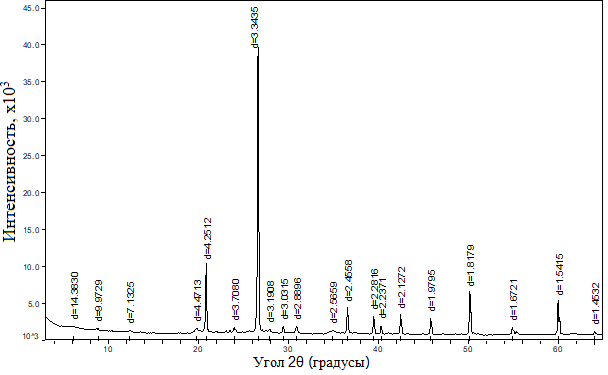
\includegraphics[scale=1.1]{dif68B7.png}
    }
    \caption{Рентгеновская дифракционная картина образца GJ68B7.}\label{fig:fig}
  \end{figure}

  \begin{figure}[ht]
    \centerfloat{
      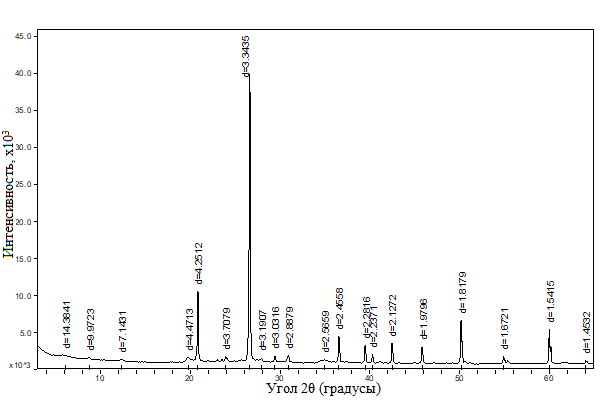
\includegraphics[scale=1.1]{dif68D4.png}
    }
    \caption{Рентгеновская дифракционная картина образца GJ68D4.}\label{fig:fig}
  \end{figure}

  \begin{figure}[ht]
    \centerfloat{
      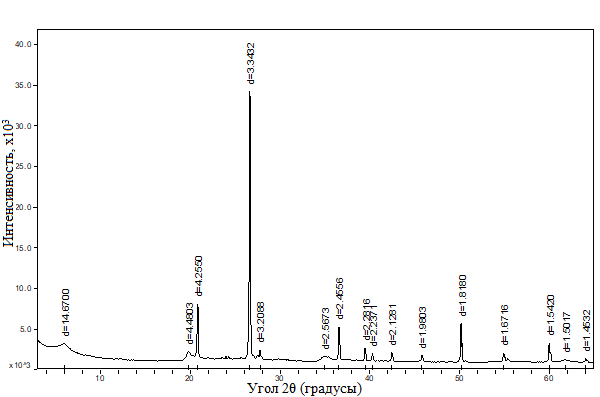
\includegraphics[scale=1.1]{dif6890.png}
    }
    \caption{Рентгеновская дифракционная картина образца GJ6890.}\label{fig:fig}
  \end{figure}

  \begin{figure}[ht]
    \centerfloat{
      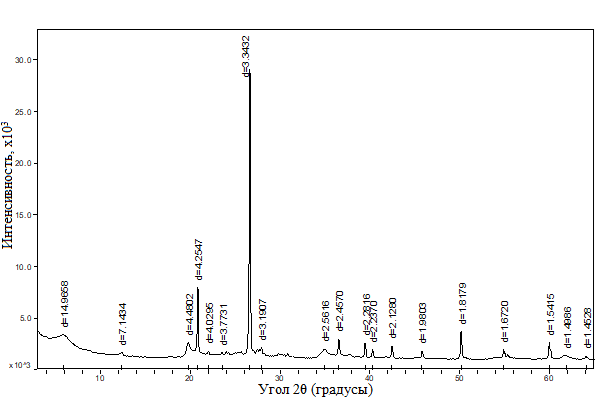
\includegraphics[scale=1.1]{dif6881.png}
    }
    \caption{Рентгеновская дифракционная картина образца GJ6881.}\label{fig:fig}
  \end{figure}

  \begin{figure}[ht]
    \centerfloat{
      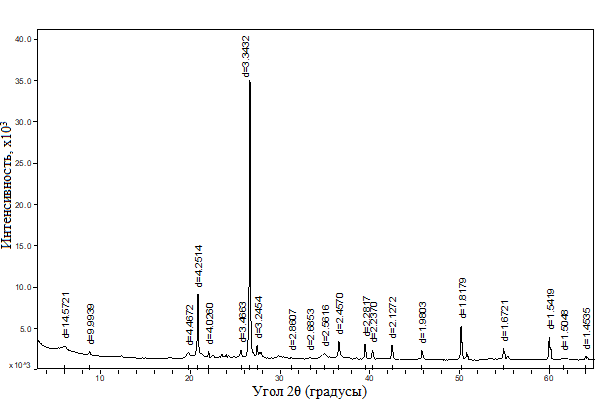
\includegraphics[scale=1.1]{dif6898.png}
    }
    \caption{Рентгеновская дифракционная картина образца GJ6898.}\label{fig:fig}
  \end{figure}

  \begin{figure}[ht]
    \centerfloat{
      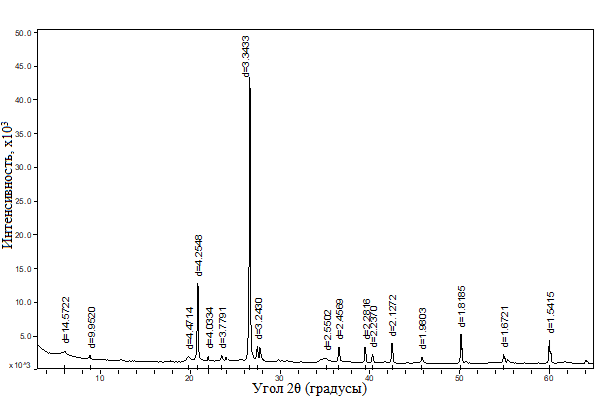
\includegraphics[scale=1.1]{dif6899.png}
    }
    \caption{Рентгеновская дифракционная картина образца GJ6899.}\label{fig:fig}
  \end{figure}